\todo[inline]{Einleitung}

%%%%%%%%%%
\section{Architektur des Moodle-Plugins}
\label{sec:architektur}
Bei der Implementierung des Hyperaudio-Plugins ist die durch Moodle vorgegebene Architektur von Plugins zu beachten \citep{moodle2016activity}. Diese besteht stets aus vorgegebenen Dateien und Ordnen, wobei die jeweilige Anzahl von der Art des zu entwickelnden Plugins abhängig ist. Darüber hinaus bestimmt die Art des Plugins auch den zu wählenden Speicherort.

Bei Activity Plugins, wie dem Plugin für Hyperaudio-Dokumente, ist als Speicherort der Ordner \textbf{/mod} vorgeben. In diesem Ordner muss ein Unterordner mit dem Namen des Plugins angelegt werden, in diesem Fall \textbf{hyperaudio}, in welchem alle Plugin-Dateien abgelegt werden. Eine Übersicht über die Ordnerstruktur des Hyperaudio-Plugins findet sich in Abbildung \ref{fig:Ordnerstruktur}.

\begin{figure}[h!]
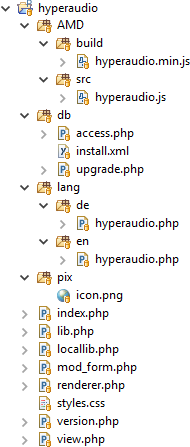
\includegraphics[width=0.3\textwidth,center]{Ordnerstruktur.PNG}
\caption{\label{fig:Ordnerstruktur}Ordnerstruktur des Hyperaudio-Plugins}
\end{figure}

\todo[inline]{Ordnerstruktur aktualisieren}

Im Ordner \textbf{/hyperaudio/backup} werden die Dateien abgelegt, welche Anwendung finden, wenn ein Backup oder eine Wiederherstellung eines Kurses vorgenommen wird.

Der Ordner \textbf{/hyperaudio/db} beherbergt die Dateien \textbf{access.php}, \textbf{events.php}, \textbf{install.xml} und \textbf{upgrade.php}. Die Datei \textbf{access.php} dient zur Steuerung der Berechtigungen innerhalb des Moodle-Plugins, wobei den verschiedenen Moodle-Rollen verschiedene Rechte für die einzelnen Funktionen zugewiesen werden können. In der \textbf{events.php} können Beobachter eingerichtet werden, welche auf bestimmte Ereignisse warten. Bei der Installation des Plugins wird die \textbf{install.xml} zur Erstellung der Datenbanktabellen für das Plugin verwendet. Es ist mindestens eine Tabelle mit dem Namen des Plugins anzulegen. Sollten die Datenbanktabellen nach Veröffentlichung des Plugins um Spalten erweitert werden, so kommt die Datei \textbf{upgrade.php} zum Einsatz. Hierin werden die notwendigen Schritte für einen Versionsabgleich definiert.

Im Ordner \textbf{/hyperaudio/lang} wird die Sprachlokalisierung vorgenommen. Für jede Sprache wird innerhalb des \textbf{lang}-Ordners ein eigener Unterordner angelegt. Darin befindet sich jeweils eine PHP-Datei, in welcher die Übersetzungen definiert werden. Der Name dieser Datei entspricht wiederum dem Namen des Plugins.

Das Icon, welches für das Plugin  verwendet werden soll, muss im Ordner \textbf{/hyperaudio/pix} mit dem Dateinamen \textbf{icon.gif} abgelegt werden und sollte eine Auflösung von 16x16 Pixel besitzen.

Im Ordner \textbf{/hyperaudio} liegen darüber hinaus die Dateien \textbf{lib.php}, \textbf{mod\underline{{ }}form.php}, \textbf{index.php}, \textbf{view.php} und \textbf{version.php}. Die \textbf{lib.php} dient dazu, Standardfunktionen von Moodle zu überschreiben, wobei \texttt{add\underline{{ }}instance}, \texttt{update\underline{{ }}instance} und \texttt{delete\underline{{ }}instance} als essenzielle Funktionen zu nennen sind. Mit diesen Funktionen wird das Anlegen, Aktualisieren und Löschen von Instanzen des Plugins ermöglicht. Zum Anlegen und Aktualisieren wird in der \textbf{mod\underline{{ }}form.php} die dazugehörige Maske festgelegt.


\textbf{\textit{index.php}}

\todo[inline]{index.php}

Die \textbf{view.php} ist die erste Datei, die beim Öffnen der Aktivität geladen wird und dient dementsprechend vornehmlich der Anzeige der Inhalte. In der \textbf{version.php} wird die Version des Plugins gepflegt. Erhöht sich die Versionsnummer in der \textbf{version.php}, wird der automatische Upgradeprozess von Moodle für das Plugin ausgelöst.

\todo[inline]{Best Practices - weitere Dateien: styles.css, renderer.php, locallib.php, ...}

%%%%%%%%%%
\section{Iterative Entwicklung}
Die Entwicklung des Plugins wird in iterativer Form durchgeführt. In jeder Iteration soll das Plugin nur um einige wenige Funktionalitäten erweitert werden. Jede Iteration soll mit einem lauffähigen Plugin abgeschlossen werden. So kann direkt das Ergebnis betrachtet werden und gegebenenfalls in der nächsten Iteration nochmals angepasst werden \citep{augsten2018iterativ}.

\subsection{Speichern und Abspielen einer Audio-Datei}
In der ersten Iteration wird zunächst die grundlegende Struktur des Plugins erstellt (vgl. Abschnitt \ref{sec:architektur}). Ziel der ersten Iteration soll es sein, eine Audio-Datei speichern und wiedergeben zu können.

Dazu wird in der Maske zum Anlegen und Aktualisieren von Instanzen des Hyperaudio-Plugins (\textbf{mod\underline{{ }}form.php}), neben dem obligatorischen Namens-Feld noch ein Element zum Hinzufügen einer Audiodatei angelegt. Auflistung \ref{lst:it1:modform} zeigt einen Ausschnitt des Codes, der in der Funktion \texttt{definition} der Klasse \texttt{mod\underline{{ }}hyperaudio\underline{{ }}mod\underline{{ }}form}, die von der Klasse \texttt{moodleform\underline{{ }}mod} erbt, ergänzt werden muss. 

\begin{lstlisting}[language=php,
             linewidth=\textwidth,
             caption={Ausschnitt der \textbf{mod\underline{{ }}form.php} in der 1. Iteration},
             label={lst:it1:modform}]
$mform = $this->_form;             
$mform->addElement('text', 'name', get_string('hyperaudio_mod_form_name',
    'hyperaudio'));
$mform->setType('name', PARAM_TEXT);
$mform->addRule('name', get_string('error_wrong_hyperaudio_name_input',
    'hyperaudio'), 'required');
$mform->addElement('filemanager', 'audiofile', get_string('hyperaudiodata',
    'hyperaudio'), null,
    array(
       'subdirs' => 0,
       'maxbytes' => 0,
       'areamaxbytes' => 10485760,
       'maxfiles' => 1,
       'accepted_types' => array('audio')
    )
);
$mform->addRule('audiofile', get_string('required', 'hyperaudio'), 'required');
\end{lstlisting}

Der \texttt{\underline{{ }}form} der \texttt{moodleform\underline{{ }}mod} können durch \textit{addElement} neue Form-Elemente hinzugefügt werden. Mithilfe der Funktionen \texttt{setType} und \texttt{addRule} können den Elementen Datentypen und Regeln zugewiesen werden, die bei Auswertung der Form automatisch validiert werden.
% im Fall von \textit{name} der Typ \textit{PARAM_TEXT} und die Bedingung \textit{required}.
Zum Hochladen von Dateien kann der \textit{filemanager} eingesetzt werden. Mithilfe eines Arrays können dabei Einschränkungen für Anzahl und Eigenschaften der hochzuladenden Dateien festgelegt werden, in diesem Fall darf maximal eine Datei hinzugefügt werden, die vom Typ \textit{audio} sein muss. Die Funktion \texttt{get\underline{{ }}string} dient im Allgemeinen der Darstellung der lokalisierten Bezeichnungen.

Um die Daten aus der Form in der Datenbank speichern und später wieder löschen zu können, muss auch die \textbf{lib.php} bearbeitet werden. Dazu dienen die bereits erwähnten Funktionen \texttt{add\underline{{ }}instance}, \texttt{update\underline{{ }}instance} und \texttt{delete\underline{{ }}instance}. Beispielhaft wird in Auflistung \ref{lst:it1:lib} die Funktion \texttt{add\underline{{ }}instance} zum Hinzufügen eines neuen Hyperaudio-Dokuments betrachtet. 

\begin{lstlisting}[language=php,
             linewidth=\textwidth,
             caption={Ausschnitt der \textbf{lib.php} in der 1. Iteration},
             label={lst:it1:lib}]
function hyperaudio_add_instance($data) {
    global $DB;
    
    $cmid = $data->coursemodule;
    $context = context_module::instance($cmid);
    
    $draftitemid_audiofile = $data->audiofile;
    unset($data->audiofile);
     
    $now = time();
    $data->timecreated = $now;
    $data->timemodified = $now;
    
    $data->id = $DB->insert_record('hyperaudio', $data);
    
    hyperaudio_update_audiofile($data->id, $context, $draftitemid_audiofile);
     
    return $data->id;
}
\end{lstlisting}

Der Parameter \texttt{\$data} enthält bereits die in der Form eingegebenen Daten. Das Attribut \mbox{\texttt{audiofile}} enthält nicht die Audio-Datei selbst, sondern die ID der \textit{draft file area} und soll im ersten Schritt nicht in der Tabelle \textit{hyperaudio} abgespeichert werden (vgl. Zeilen 7-8). Vor dem Speichern wird noch der aktuelle Zeitstempel hinterlegt (vgl. Zeilen 10-12). Mithilfe der Funktion \mbox{\texttt{\$DB->insert_record}} kann das \texttt{\$data}-Objekt mit seinen Attributen in der Tabelle \textit{hyperaudio} abgelegt werden. Im Nachhinein sorgt die in der \textbf{locallib.php} definierte Funktion \mbox{\texttt{hyperaudio_update_audiofile}} dafür, dass die Audio-Datei in der \textit{files}-Tabelle abgespeichert und in der \textit{hyperaudio}-Tabelle korrekt referenziert wird (vgl. Auflistung \ref{lst:it1:locallib}).

\begin{lstlisting}[language=php,
             linewidth=\textwidth,
             caption={Ausschnitt der \textbf{locallib.php} in der 1. Iteration},
             label={lst:it1:locallib}]
function hyperaudio_update_audiofile($hyperaudioid, $context, $draftitemid) {
    global $DB;
    
    file_save_draft_area_files($draftitemid, $context->id, 'mod_hyperaudio',
    'audiofile', $hyperaudioid);
    $fs = get_file_storage();
    $files = $fs->get_area_files($context->id, 'mod_hyperaudio', 'audiofile',
    $hyperaudioid, 'itemid, filepath, filename', false);

    $file = reset($files);
    $DB->set_field('hyperaudio', 'audiofile', $file->get_filename(), array(
        'id' => $hyperaudioid
    ));
}
\end{lstlisting}

Wie bereits in Abschnitt \ref{sec:architektur} angedeutet, übernimmt die \textbf{renderer.php} die Anzeige der Hyperaudio-Inhalte (siehe Auflistung \ref{lst:it1:renderer}). Die \textbf{view.php} dagegen reduziert sich auf wenige Zeilen (vgl. Auflistung \ref{lst:it1:view}). Der Plugin-Renderer wird hier benutzt, um Header, Hauptinhalte und Footer anzuzeigen.

\begin{lstlisting}[language=php,
deletekeywords={header},
             linewidth=\textwidth,
             caption={Ausschnitt der \textbf{view.php} in der 1. Iteration},
             label={lst:it1:view}]
$output = $PAGE->get_renderer('mod_hyperaudio');
echo $output->header();
echo $output->display($hyperaudio, $context);
echo $output->footer();
\end{lstlisting}

In der Funktion \texttt{display} der Klasse \mbox{\texttt{mod_hyperaudio_renderer}}, die von der Klasse \mbox{\texttt{plugin_renderer_base}} erbt, werden die HTML-Inhalte erzeugt. Dabei handelt es sich in der 1. Iteration um einen Container, der ein \texttt{<audio>}-Element beinhaltet. Als Quelle wird im \texttt{<source>}-Element eine URL (Uniform Resource Locator) angegeben, die zuvor mit Moodle-Standardmitteln erzeugt wurde und auf die in der Datenbank abgelegte Audio-Datei verweist.

\begin{lstlisting}[language=php,
             linewidth=\textwidth,
             caption={Ausschnitt der \textbf{renderer.php} in der 1. Iteration},
             label={lst:it1:renderer}]
$audio_fileinfo = array(
    'component' => 'mod_hyperaudio',
    'filearea' => 'audiofile',
    'itemid' => $hyperaudio->id,
    'contextid' => $context->id,
    'filepath' => '/',
    'filename' => $hyperaudio->audiofile
);

$audiofileurl = moodle_url::make_pluginfile_url(
    $audio_fileinfo['contextid'], $audio_fileinfo['component'],
    $audio_fileinfo['filearea'], $audio_fileinfo['itemid'],
    $audio_fileinfo['filepath'], $audio_fileinfo['filename']);
$audio_url = $audiofileurl->get_port() ? $audiofileurl->get_scheme() . '://' .
    $audiofileurl->get_host() . $audiofileurl->get_path() . ':' .
    $audiofileurl->get_port() : $audiofileurl->get_scheme() . '://' .
    $audiofileurl->get_host() . $audiofileurl->get_path();

$output = '<div id="hyperaudio" data-hyperaudio_id="'.$hyperaudio->id.'">';
$output .= '<audio id="hyperaudio_audio" controls style="width:800px;">' .
    '<source src="' . $audio_url . '"/>' .
    '</audio>';
$output .= '</div>';

echo $output;
\end{lstlisting}

Auf die beschriebene Art und Weise lässt sich ein Hyperaudio-Dokument, das vorläufig allein aus einer Audio-Datei besteht, speichern und mithilfe des HTML5-Audio-Players wiedergeben.


\subsection{Speichern und Anzeige von Zusatzinhalten}
\dots

\subsection{Einbindung der Konfigurationsdatei}
\dots

\subsection{Speichern und Anzeige von Kommentaren}
\dots

\subsection{Antworten auf Kommentare}
\dots

\subsection{Galerie der Zusatzinhalte}
\dots

\subsection{Visualisierung der Annotationen in der Timeline}
\dots

%%%%%%%%%%
\section{Zusammenfassung}
\dots